\documentclass[bibtotocnumbered, headsepline,normalheadings,12pt,polish]{scrreprt}
\usepackage[T1]{fontenc}
\usepackage[utf8]{inputenc}
\usepackage{geometry}
\geometry{tmargin=25mm,bmargin=25mm,lmargin=30mm,rmargin=30mm}
\usepackage{babel}
\setlength\parindent{0pt}
\usepackage{graphics}
\usepackage{floatflt}
\usepackage{scrpage}
\usepackage{alltt}
\usepackage{pdfpages}
\usepackage{hyperref}
\usepackage{moreverb}

\usepackage{booktabs}
\usepackage{array}
\usepackage{listings}
\lstset{breaklines=true}

\pagestyle{headings}
\begin{document}
\title{\textbf{Dokumentacja programu zarządzającego bazą studentów, prowadzących i przedmiotów}}
\date{}
\maketitle

\tableofcontents

\chapter{Wstęp}
\section{Opis Problemu}
\large
Celem projektu jest jest napisanie programu, który będzie zarządzał bazą danych zawierającą studentów, przedmioty i prowadzących. Funkcje implementujące działanie programu zostaną oddzielone od interfejsu użytkownika, w celu umożliwienia udostępnienia ich jako biblioteka.

Program będzie potrafił obsługiwać bazy danych o teoretycznie dowolnej wielkości dzięki wczytywaniu plików we fragmentach.

\section{Narzędzia}
\large
Program został napisany w języku\texttt{ \textbf{C}} zgodnym ze standardem \textbf{ISO C90}.
Wykorzystywano kompilator \textbf{gcc}, debugger \textbf{gdb}.
Program jest konfigurowany i budowany przy użyciu \textbf{GNU Autotools} i \textbf{GNU Make}.
Dokumentacja jest formatowana przy użyciu \texttt{\textit{LaTeX}.}

\chapter{Specyfikacja Funkcjonalna}
\section{Funkcjonalność}
\subsection{Funkcjonalność podstawowa}
\begin{itemize}
\item dodawanie, usuwanie, edycja, wyliczanie oraz wyliczanie powiązań studentów
\item dodawanie, usuwanie, edycja, wyliczanie oraz wyliczanie powiązań prowadzących
\item dodawanie, usuwanie, edycja, wyliczanie oraz wyliczanie powiązań przedmiotów
\end{itemize}


\section{Komunikacja z użytkownikiem}
Komunikacja z użytkownikiem odbywa się w trybie wsadowym przez tekstowy interfejs użytkownika.

\subsection{Argumenty lini poleceń}
\pagebreak
\verbatimtabinput[4]{man_tester}
\large

\subsection{Plik konfiguracyjny}
Argumenty lini poleceń mogą zostać zapisane w pliku \begin{verbatim}~/.spprc\end{verbatim} 
(lub innym podanym przy opcji --config). Będą one wczytywane przy każdym wywołaniu programu bez konieczności podawania ich z lini komend. Przykładowy plik konfiguracyjny:
\normalsize
\begin{verbatim}
#------------------------------
--log log.txt                   # komunikaty diagnostyczne do log.txt
--data ~/db                     # lokalizacja bazy danych
#---------------EOF------------
\end{verbatim}
\small
\subsection{Przykłady użycia programu}

\begin{verbatim}
# dodanie przedmiotu
spp --type subject --add --name "Programowanie" \
--subject-type "egz" --hours "30" --date "Piątek 18:15"

spp --type subject --add --name "Wychowanie Fizyczne" \
--subject-type "zal" --hours "30" --date "Poniedziałek 8:15"

# dodanie studenta
spp --type student --add --name "Janek Kowalski" \
--index 123456 --subject "1,2"

# dodanie prowadzącego
spp --type lecturer --add --name "Janusz Kowalski" \
--degree "dr. hab. prof. nzw." --room "GE510" --subject "1"

# wyliczaj studentów
spp --type student --cat

# edytuj studenta
spp --type student --id 5 --edit --subject "2,3,4"

# drukuj przedmioty asocjowane ze studentem
spp --type student --id 5 --show-links

# usuń studenta
spp --type student --id 5 --rm
\end{verbatim}
\large
\section{Format Danych}
\subsection{Baza danych}
Dane będa przechowywane w prostej bazie danych. Przykładowy rekordy:\\
\begin{itemize}
\normalsize
\item student
\begin{verbatim}
    id|name|indeks|subjects
    --------------------------------------------
    5|Janek Kowalski|123456|Programowanie, Wychowanie fizyczne
\end{verbatim}
\item prowadzący
\begin{verbatim}
    id|name|degree|room|subjects
    --------------------------------------------
    5|Janusz Kowalski|dr. hab. prof. nzw.|GE510| Programowanie, Bazy danych
\end{verbatim}
\item przedmiot
\begin{verbatim}
    id|name|subject type|hours|date
    --------------------------------------------
    5|Programowanie|egz|30|Piątek 18:15
\end{verbatim}
\end{itemize}
\subsection{Dane wyjściowe}
\large
\begin{itemize}
\item program standardowo wyświetla jeden rekord na linię
\item wszystkie komunikaty poprzedzone są znakiem "!" i wypisywane na stderr lub do loga
\subitem * komunikaty ostrzegawcze " ! W "
\subitem * komunikaty fatalne      " ! E "
\subitem * możliwe jest zwiększenie ilości wypisywanych komunikatów diagnostycznych przez dodanie flagi --verbatim
\end{itemize}

\section{Działanie w przypadku nieprawidłowych danych}
Program stara się testować argumenty. W przypadku podania przez użytkownika nieprawidłowych danych program przerywa działanie oraz wypisuje kod błędu.


\normalsize

\chapter{Specyfikacja Implementacyjna}
\section{Opis Ogólny}


Krótki opis modułów.\\
\begingroup
  \setlength\tabcolsep{3pt}
  \small
  \begin{tabular}{|b{1in}|b{1in}|b{1in}|r|}
    \toprule
    {\bfseries Moduł} &  {\bfseries Pliki} & {\bfseries Zależy} & {\bfseries Opis} \\
    \midrule
    \hline
{\bfseries Baza \newline danych}\\
    \hline
    db & db\_io.[ch] dbtypes.h & util & prosta baza danych\\
    \midrule
    spp & spp.c\newline spp.h & db util  & eksportuje funkcjonalność bazy danych \\\midrule
    util & util.c \newline util.h & - & funkcje pomocnicze\\\midrule
    define& define.h & - & lokalne stałe\\\midrule
    \hline
{\bfseries Interfejs \newline Użytkownika}\\
    \hline
    ui\_text & ui\_text.c ui\_text.h & spp & tekstowy interfejs użytkownika \\\midrule
    \midrule
  \end{tabular}
\endgroup
\large
\\ \\ \\
Program korzysta z następujących systemowych plików nagłówkowych:
\begin{itemize}
\item stdlib.h
\item stdio.h
\item string.h
\item time.h
\item stdarg.h
\item getopt.h
\item ctype.h
\end{itemize}

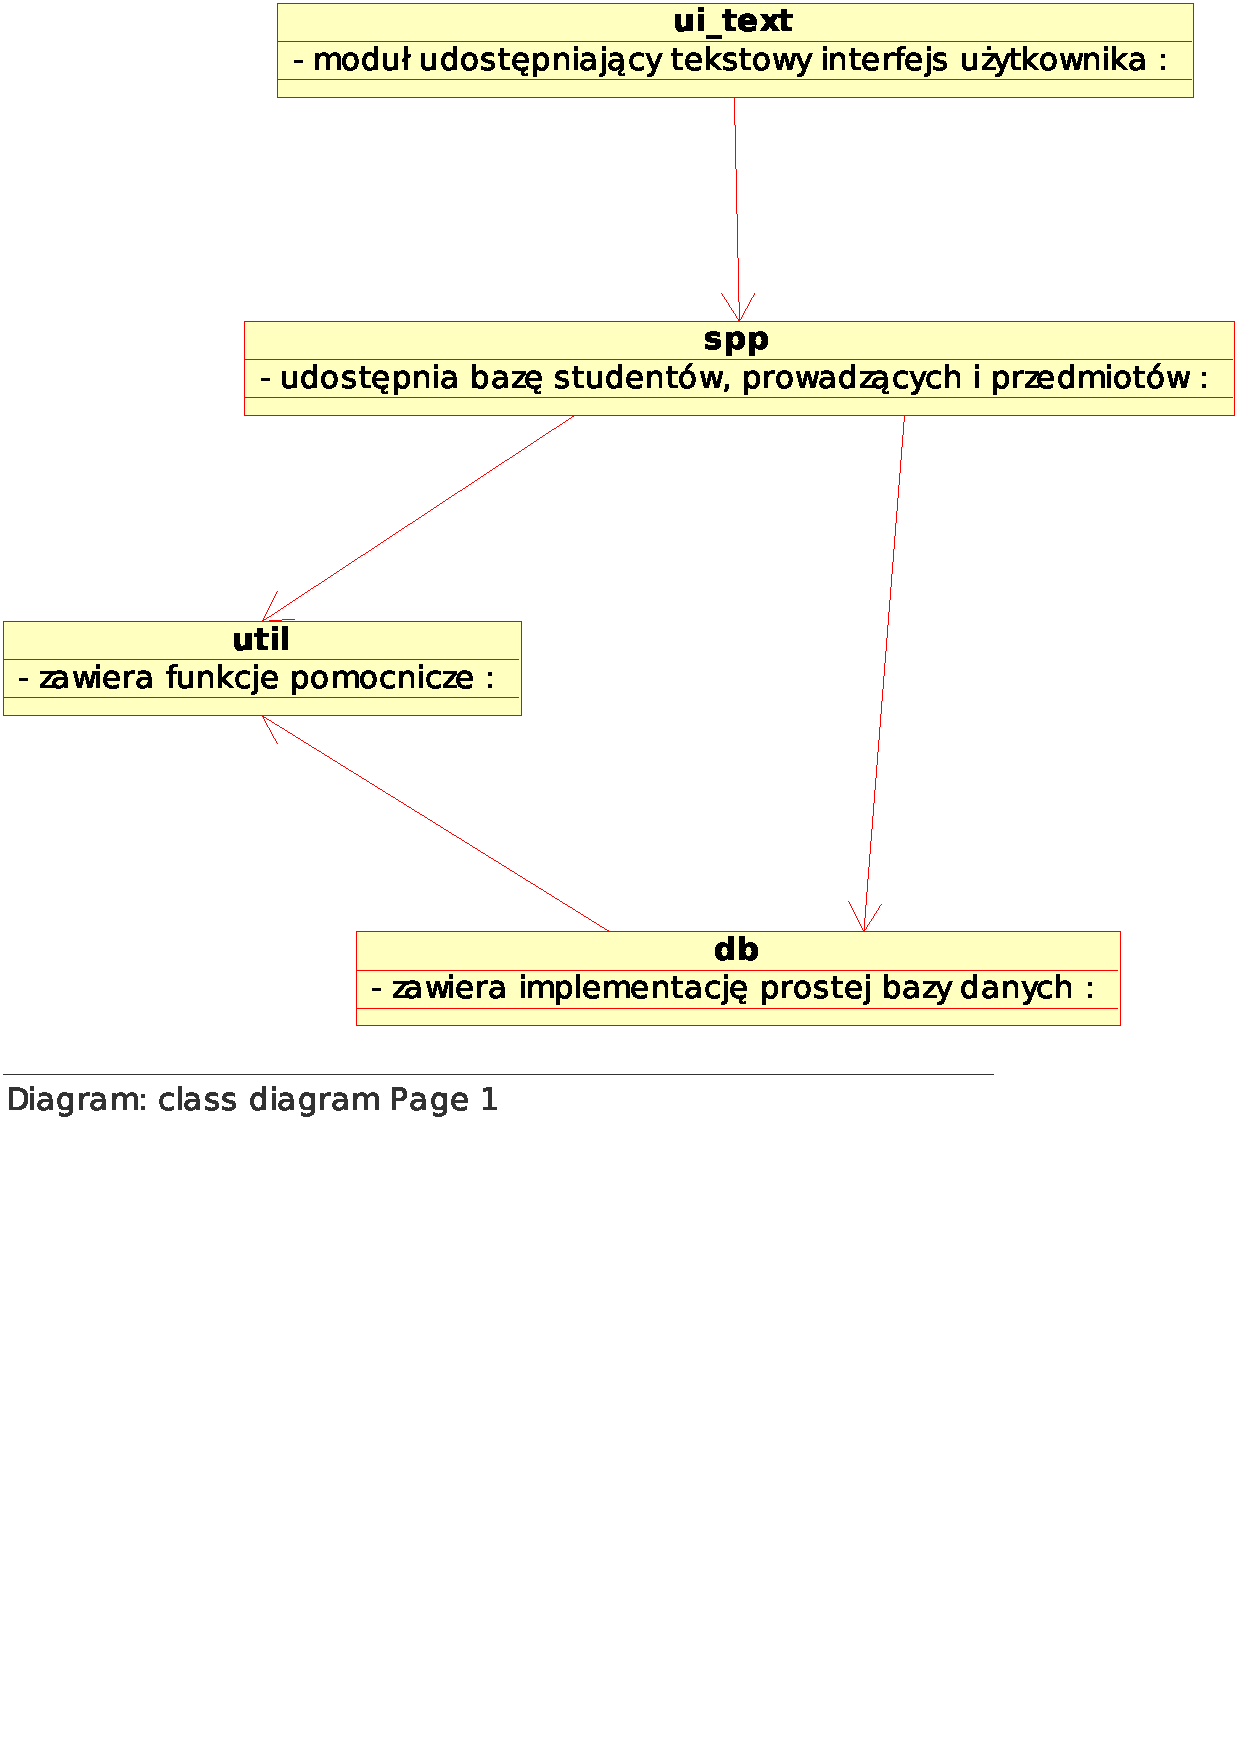
\includepdf[fitpaper,pages=1]{spp_diagram_modulow.pdf}

\section{Baza danych}
Baza danych jest przechowywana w trzech plikach tekstowych:
\begin{itemize}
\item *.stud - rekordy studentów
\item *.lecturer - rekordy prowadzących
\item *.topic - rekordy przedmiotów
\end{itemize}
Maksymalna liczba rekordów jednorazowo wczytywanych przez bazę danych jest określona poprzez MAX\_RECORDS ( domyślnie 10 ). Po wykonaniu operacji następuje wczytanie kolejnych rekordów z bazy danych. Dzięki takiej implementacji, wielkość wymaganej pamięci operacyjnej nie zwiększa się wraz z wiekością bazy danych.
Rekordy są indeksowane od 1 ( dla każdego pliku oddzielnie). Rekordy studentów i prowadzących są powiązane z rekordami przedmiotów poprzez indeksy odseparowane przecinkami, które są wczytywane do pola \textbf{topic}. Usunięcie przedmiotu powoduje również usunięcie powiązań znajdujących się w rekordach studentów i prowadzących.
W pliku db\_types.h znajdują się definicje struktur danych:
\begin{verbatim}
typedef struct _st_rekord_lecturer
{
    int id;
    char name[MAX_NAME];
    char degree[MAX_DEGREE];
    char room[MAX_ROOM];
    char topic[MAX_TOPIC];
} st_rekord_lecturer;

typedef struct _st_rekord_topic
{
    int id;
    char name[MAX_NAME];
    char topic_type[MAX_TOPIC_TYPE];
    int hours;
    char date[MAX_DATE];
} st_rekord_topic;

typedef struct _st_rekord_student
{
    int id;
    char name[MAX_NAME];
    int index;
    char topic[MAX_TOPIC];
} st_rekord_student;
\end{verbatim}


Baza danych udostępnia swoją funkcjonalność przez moduł spp.
\subsection{Moduł spp}
\large
Moduł \textbf{spp} składa się z 2 plików: \textit{\textbf{spp.c spp.h}}\\
\textbf{spp} daje dostęp do bazy danych przez prosty interfejs\\
\textbf{spp} jest zależny od \large modułów \emph{db , util}.\large\\
Potrzebuje definicje stałych zawarte w pliku \large\emph{define.h}.\large\\

\textbf{spp} składa się z następujących elementów:
\begin{verbatim}
/* Struktura sppArgs zawiera wszystkie~
 * parametry potrzebne modułowi spp */
struct sppArgs
{
    int mode; /* tryb działania */

    char type; /* typ rekordu na którym operujemy */
    char *data; /* nazwa bazy danych */
    char *log; /* nazwa pliku logu */
    char *out; /* plik wyjścia standardowego */
    char *build; /* nazwa tworzonej bazy danych */

    int id; /* pole rekordu: numer identyfikacyjny rekordu */
    char *name; /* pole rekordu: nazwa */
    char *degree; /* pole rekordu: stopień naukowy */
    char *room; /* pole rekordu: pokój */
    char *date; /* pole rekordu: termin zajęć */
    char *topic; /* pole rekordu: przedmioty */
    char *topic_type; /* pole rekordu: typ przedmiotu */
    int hours; /* pole rekordu: liczba godzin */
    int index; /* pole rekordu: numer indeksu */
};

/* Funkcja przygotowująca moduł spp do działania, 
 * jako argument pobiera struckturę sppArgs.
 * Kody błędów powyżyej. */
int 
spp_setup (struct sppArgs *);

/* Funkcja kończąca działanie modułu spp.
 * Zamyka pliki i uwalnia pamięć
 * Kody błędów powyżyej. */
void 
spp_finish ();

/* Wywołanie funkcji spp_run powoduje wykonanie
 * działań zaprogramowanych w strukturze sppArgs
 * Kody błędów powyżyej. */
int spp_run ();
\end{verbatim}
\subsection{Moduł db}
\large
Moduł \textbf{db} składa się z 3 plików: \textit{\textbf{db\_io.c db\_io.h dbtypes.h }}\\
\textbf{db} zawiera implementacje prostej bazy danych.\\
\textbf{db} jest zależny od \large modułu \emph{util}.\large\\
Potrzebuje definicje stałych zawarte w pliku \large\emph{define.h}.\large\\

Funkcjonalność udostępniana przez moduł db jest zadeklarowana w pliku db\_io.h
\begin{verbatim}
/* Funkcje wczytujące z plików (parametr FILE * in) zbiory rekordów.
 * Wynik zapisywany jest w tablicach struktur.
 *  Parametr max to maksymalna ilosc rekordów wczytana jednorazowo.
 * Funkcje zwracają liczbę wczytanych rekordów.
 */
int db_read_records_students (FILE * in, st_rekord_student records[], int max, bool * overflow);

int db_read_records_lecturers(FILE * in, st_rekord_lecturer records[], int max, bool * overflow);

int db_read_records_topics (FILE * in, st_rekord_topic records[], int max, bool * overflow);

/* Funkcje zapisujące w plikach (FILE * out) rekordy przechowywane
 * w tablicach struktur podawanych jako parametr funkcji.
 * int n - liczba rekordow w tabeli
 */

void db_write_records_students (FILE * out, st_rekord_student records[], int n);

void db_write_records_lecturers(FILE * out, st_rekord_lecturer records[], int n);

void db_write_records_topics (FILE * out, st_rekord_topic records[], int n);


/* Generuje niewykorzystany ID dla rekordu */
int dbGetNewID (FILE * in);

/* Usuwa rekord o podanym ID, wynik zapisuje w out */
int dbRemoveID(FILE * in, FILE * out, int rmid);

int db_remove_topic_id_from_stud(FILE * in, FILE * out, int rmid);

int db_remove_topic_id_from_lecturer(FILE * in, FILE * out, int rmid);
\end{verbatim}

\subsection{Moduł util}
\large
Moduł \textbf{util} składa się z 2 plików: \textit{\textbf{util.c util.h}}\\
\textbf{util} zawiera funkcje pomocnicze
\textbf{util} nie zależy od innych modułów.\\
Potrzebuje definicje stałych zawarte w pliku \large\emph{define.h}.\large\\

\textbf{util} składa się z następujących elementów:
\begin{verbatim}

/* Funkcja kopiująca pliki. 
 * Zwraca 0 lub wartość != 0 dla niepowodzenia */
int 
util_copy_file(FILE *in, FILE *out);

/* Funkcja usuwająca znak nowej lini. 
 * Zwraca wskaźnik na wynikowy łańcuch znaków */
char * 
util_strip_nl(char *s);

\end{verbatim}

\section{Interfejs użytkownika}
Program działa w trybie tekstowym, a komunikacja z użytkownikiem odbywa się w trybie wsadowym. Nakładka tekstowa wykorzystuje bibliotekę getopt do czytania argumentów lini poleceń.
\subsection{Moduł ui\_text}
\normalsize
Moduł \textbf{ui\_text} składa się z 2 plików: \textit{\textbf{ui\_text.c ui\_text.h}}\\
\textbf{ui\_text} zawiera funkcje nakładki tekstowej\\
\textbf{ui\_text} jest zależny od \large modułu \emph{spp}.\large\\
Potrzebuje definicje stałych zawarte w pliku \large\emph{define.h}.\large\\

\textbf{ui\_text} składa się z następujących elementów:
\begin{verbatim}

/* Funkcja kontrolująca działanie nakładki tekstowej. */
int 
ui_run (int argc, char **argv);

/* Wczytaj argumenty lini poleceń */
int 
ui_setup_arguments (int argc, char **argv);

/* Wypisz wszystkie dostępne opcje */
void 
ui_show_options (FILE *);

/* Pokaż opis programu */
void 
ui_show_description (FILE *);

/* Pokaż krótka pomoc */
void 
ui_show_help (FILE *);

\end{verbatim}
\subsection{Plik define.h}
\large
W pliku \textbf{define.h} znajdują się definicje stałych potrzebnych w programie oraz definicja typu \textit{bool}.

\section{Kody błędów}
\begin{verbatim}
Tablica kodów błędów:

-1 - złe/niewystarczające argumenty

 0 - nie wykryto błędów

 1 - nie otrzymano struktury sppArgs

 2 - wymagana nazwa pliku jest nieznana

 3 - nie udało się otworzyć pliku bazy danych

 4 - nie udało się otworzyć pliku logu
 
 5 - nie udało się otworzyć pliku wyjścia
 
 6 - nie udało się otworzyć pliku do zakodowania
 
 7 - nie udało się otworzyć pliku do odkodowania
 
 10 - błąd podczas czytania pliku
 
 11 - błąd podczas zapisywania do pliku
 
 111 - zbyt długie dane wejściowe
\end{verbatim}

\chapter{Testy}
\normalsize
\section{Kompilacja}
System operacyjny: Linux 2.6.24-21
Kompilator: gcc 4.2.4
\section{Działanie programu}
Działanie programu testowano manualnie.
Przykładowe testy (plik tests.sh):
\verbatimtabinput[8]{../tests.sh}
\section{Zgodność z założeniami}
Program działa tak jak założono podczas analizy przedprojektowej.
\end{document}
